
\documentclass{article}

\usepackage{amsmath}
\usepackage{amssymb} % for \mathbb
\usepackage{graphicx}
\usepackage{times}
\usepackage[hyperfootnotes=false]{hyperref}

\newcommand{\R}{\ensuremath{\mathbb{R}}}
\newcommand{\foreach}{\forall}

\title{%
Using Laplace's Equation to Fill a Bounded Region of a Monochromatic Image%
}

\author{Thomas E. Vaughan}

\begin{document}

\maketitle

\begin{abstract}
   I present, for a monochromatic image and by way of Laplace's Equation
   applied to information at the boundary of a connected region of pixels in
   the image, an algorithm that fills the region.  The algorithm smoothly
   propagates not only the intensity but also noise from the boundary to pixels
   in the interior of the region.

   Let $M$ be the set of pixels in a monochromatic image.  Consider any proper
   subset $N \subsetneq M$.  Let $B_N$ be the external boundary of $N$, so that
   every pixel $q \in B_N$ shares an edge with some pixel $p \in N$, but $q
   \notin N$.  Let $T_N = N \cup B_N$ be the union of $N$ and its external
   boundary $B_N$.  Let $S \subsetneq M$ be any proper subset of $M$ such that
   $T_S \subsetneq M$ is also a proper subset.  For any pixel $p \in M$, let
   $v_p$ be the original value of $p$.

   The algorithm computes a new value $r_p$ for each pixel $p \in S$.  The new
   value $r_p$ is computed on the basis of a solution to each of three
   discrete-Dirichlet problems.  To wit:
   \begin{enumerate}
      \item For each pixel $p \in S$, compute the value $a_p$ of the solution
         to the discrete-Dirichlet problem for the boundary-values $\{v_q \: |
         \: q \in B_S\}$.
      \item For each pixel $p \in T_S$, compute the value $b_p$ of the solution
         to the discrete-Dirichlet problem for the boundary-values $\{v_q \: |
         \: q \in B_{T_S}\}$.
      \item For each pixel $q \in B_S$, compute the value $\sigma_q = |b_q -
         v_q|$, which is taken as an estimate of the standard deviation for
         high-spatial-frequency noise at pixel $q$.
      \item For each pixel $p \in S$, compute the value $\sigma_p$ of the
         solution to the discrete-Dirichlet problem for the boundary-values
         $\{\sigma_q \: | \: q \in B_S\}$.
      \item For each pixel $p \in S$, compute the value $r_p = a_p + n_p$,
         where $n_p$ is a random number drawn from the Gaussian distribution
         whose standard deviation is $\sigma_p$.
   \end{enumerate}
   For an image with noise on the pixel values, this approach produces a filled
   region that does not so obviously stand out to the eye as would merely using
   $r_p = a_p$ for the new value of each pixel $p \in S$.

\end{abstract}

\section{Introduction}

In early September of 2018, I helped my son, Nicholas, with his homework for a
course in partial differential equations.  He was solving the two-dimensional
version of the Dirichlet Problem: to find for a region $A$ in the plane a
function $f: A \rightarrow \R$ obeying Laplace's Equation, which can be written
for Cartesian coordinates as\footnote{%
   I use ``$\partial_x$'' to represent the operator whose meaning is ``the
   first partial derivative with respect to $x$.'' Similarly, my
   ``$\partial_x^2$'' represents the operator whose meaning is ``the second
   partial derivative with respect to $x$.'' I picked up this notation from Ron
   Kantowski, my professor in the quantum-field-theory course that I took in
   graduate school in the early 1990s at the University of Oklahoma.}
\begin{equation}
   \left[\partial_x^2 + \partial_y^2\right] f(x,y) = 0.
\end{equation}
For every point $(x,y)$ along the boundary of $A$, the function's value $f(x,y)
= \beta(x,y)$ is known and so constrains\footnote{%
   It seems to me that $\beta$ must be sufficiently smooth in some sense;
   otherwise, $f$ would not be able to satisfy Laplace's Equation near the
   boundary.}
the solution for $f$ in $A$.

While thinking about Nicholas's problem, I was reminded of a problem that I had
faced in a digital-image-processing course that I took when I was in college,
probably around 1990.  The professor had given to the students a monochromatic
image of a grassy field and the sky with some clouds.  At each of a half-dozen
or so places in the image, he had painted a roughly circular patch of pixels a
uniform shade of gray; each patch was perhaps 15 pixels across.  The homework
had been to devise an algorithm to fill in each patch so that the filled patch
would appear minimally foreign to the surrounding image.  I don't recall my
solution, but I do recall that I was not satisfied with any of my various
attempts.  I feel as though I should remember having used Laplace's Equation if
I had in fact used it, and I have no such memory.  What's more, I am certain
that I did not employ Laplace's Equation to propagate noise from the boundary
as I propose to do here.  What seems clear to me now is that I should like to
have tried Laplace's Equation.

A few days later, I worked out the basic mathematics.  While watching my
daughter, Ana, at softball practice, I was thinking about how to express
Laplace's Equation in two-dimensional, discrete, Cartesian coordinates.  As I
sat in the stands, it came to me, and I realized that I should have to solve a
sparse, linear system.

\newcommand{\mathworksurl}{https://blogs.mathworks.com/steve/2015/06/17/region-filling-and-laplaces-equation/}

The next day, I searched the Internet for information on filling a region of an
image via Laplace's Equation.  I supposed---because using Laplace's Equation
seems so obvious an approach to me now---that either the use of Laplace's
Equation is common for this application, or the solution does not work well for
one reason or another.  What I found most relevant in my search is a
\href{\mathworksurl}{blog post}\footnote{\mathworksurl} by Steve Eddins of
MathWorks.  Eddins provides some images as an example of his approach,
implemented in Matlab.

Eddins presents the Laplacian-fill approach as useful for eliminating an object
from an image. One could use a polygon-fill tool in an image-editing program to
mark a boundary around the object
\begin{figure}
   \begin{center}
   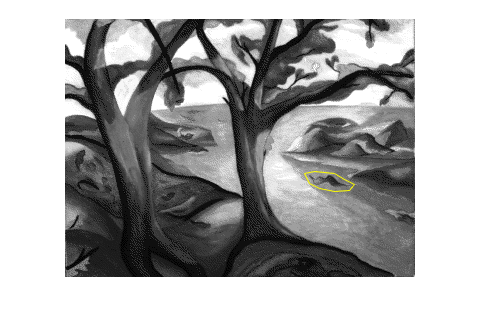
\includegraphics[width=0.99\columnwidth]{exploring_regionfill_01}
   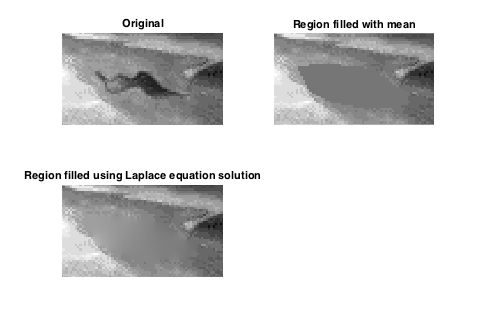
\includegraphics[width=0.99\columnwidth]{exploring_regionfill_12}
   \end{center}
   \caption{Example of Eddins. Top: Boundary drawn around object to eliminate
   from image. Bottom: Zoomed-in view of solution.}
   \label{fig:boundary}
\end{figure}
and then to fill the polygon with a uniform intensity.  See
Figure~\ref{fig:boundary}.  In his example, Eddins initially fills the polygon
with the mean intensity of the pixels originally inside the boundary.  His
final solution appears in one of the zoomed-in images at the bottom of the
figure.

\end{document}

